\chapter{Absolute Indexing Design}

Without a doubt, the multi-finger painting case projects have proven to be the most troublesome to implement using both of the two previously presented designs. It is impossible to elegantly implement a multi-finger painting project using the Closest Finger Design, because the design does not offer a method to differentiate between individual touches other than through the comparison of touch locations. The Relative Indexing Design suffers from a similar inability. Although the Relative Indexing Design makes it easy to distinguish all of the present touches (using their relative indices), the design does not enable scripts to determine when touches switch indices. As a result, it is difficult to program paintbrushes to follow specific touches, since the touches' associated indices are subject to change. If every touch were given a unique index that it kept from its creation to its end (i.e., an ID number), then it would not be difficult to distribute touches amongst the paintbrush sprites so that every touch is followed by exactly one paintbrush.

This concept, assigning each created touch a unique, permanent  number, is the main premise behind the \emph{Absolute Indexing Design}, the third and final multi-interaction set design. Touches in the Absolute Indexing Design are indexed in order of initiation relative to all touches that have been made since the inception of the project. As a result, a touch's associated index can never change in the Absolute Indexing Design, because the $n$th touch pressed in the execution of a project will forever be the $n$th touch pressed.

While the Absolute Indexing Design can facilitate the implementation of certain complex multi-touch interactions, it can make implementing simpler single-touch interactions more difficult. In this chapter, I will again first specify the design and afterwards evaluate it using the three iterations of case projects described in Chapter 3.

\section{Interaction Set Specification}

The Absolute Indexing Design consists of nine blocks (Figure \ref{FamiliarAIDBlocks}), only two of which are wholly original. In contrast to the previous chapter, I will specify the familiar blocks before presenting the newer ones.

The seven familiar blocks in the Absolute Indexing Design each have counterparts in the Relative Indexing Design, but with two main differences. The first difference between these blocks and their Relative Indexing Design counterparts is that their parameters are text inputs rather than drop-down menus. Since the touch indices are not bounded by 10 in the Absolute Indexing Design, a drop-down menu would not make sense. Also, these parameters are best thought of as (\emph{ID})s instead of (\emph{index})es. The second difference is that the term ``finger" is replaced with ``touch" in the block labels. Although the use of the term ``finger" was not perfectly suitable in the Relative Indexing Design either, the term ``finger"  makes no sense at all when using absolute indexing. For example, the term ``finger (73)" implies that the user has at least 73 fingers, whereas ``touch (73)" accurately implies the 73rd touch pressed on the tablet.

Thus, the seven familiar blocks are named: ``touch (\emph{ID}) down?", ``touching touch (\emph{ID})?", ``distance to touch (\emph{ID})," ``point towards touch (\emph{ID})," ``go to touch (\emph{ID})," ``touch (\emph{ID}) x," and ``touch (\emph{ID}) y." Functionally, these seven Absolute Indexing Design blocks work in a manner similar to their Relative Indexing Design counterparts, just with different touch indexing. For example, the ``touch (\emph{ID}) down?" block reports the value of \emph{true} if the (\emph{ID})th touch in the project's execution  has been created and is still touching the tablet and otherwise reports the value of \emph{false}. Similarly, the remaining six familiar blocks all correspond to the location of the (\emph{ID})th touch in the project's execution. If the (\emph{ID})th touch has yet to be made, its location is considered to be $\{0,0\}$. Also, if the (\emph{ID})th touch has already been both made and lifted, its location is considered to be its last touched location. If the inserted value of (\emph{ID}) is anything other than a positive integer, the location of interest is always defaulted to $\{0,0\}$.

\begin{figure}
\centering
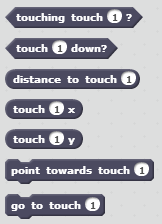
\includegraphics{images/FamiliarAIDBlocks.PNG}
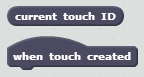
\includegraphics{images/NewAIDBlocks.PNG}
\caption[The Absolute Indexing Design Interaction Set]
{The seven familiar blocks in the Absolute Index Designs are on the left, while the two new blocks are on the right.}
\label{FamiliarAIDBlocks}
\end{figure}

Now that the familiar blocks have been specified, I will introduce the two original blocks. The first of the entirely new blocks is a function block, labeled ``current touch ID." Simply put, the ``current touch ID" block reports the unique ID of the most recently made touch. When touches have yet to be made, the ``current touch ID" block reports the value 0, since the first touch in the execution of a project has an ID of 1. An important aspect of the behavior of the ``current touch ID" is that it increases by at most 1 per execution iteration of the Scratch programming environment. In other words, if a loop in Scratch is constantly checking the value of the ``current touch ID" block at each iteration (without having inner loops or ``wait" blocks), the value will not jump from \emph{x} to \emph{x+2} without being valued as \emph{x+1} first, even if two touches are made simultaneously. Thus, it is possible to watch the ``current touch ID" block without having to worry about missing a touch.

The second new block is a trigger block labeled, ``when touch created." In many ways  the ``when touch created" block is analogous to the ``when finger pressed" block from the extended version of the Closest Finger Design and the ``when finger (\emph{index}) pressed" block from the Relative Indexing Design. However, its behavior is unique and important to the Absolute Indexing Design. Like the ``when finger pressed" block, the ``when touch created" block is triggered by the initiation of every touch. However, unlike the ``when finger pressed" block, the ``when touch created" block does not create a new thread for every touch. Instead, the ``when touch created" block handles simultaneous triggerings in a way similar to the ``current touch ID" block. If, for example, two simultaneous touches are made, the ``when touch created" block would first execute its first stack as far as it can in one Scratch execution iteration (stopping only at a ``wait" block or the end of a loop), before restarting the stack execution in the next Scratch execution iteration. Therefore, if the first block in a ``when touch created" block's connected stack contains a reference to the ``current touch ID" block, the ``current touch ID" block would have the ID of the (arbitrarily chosen) first touch during the first execution and the ID of the second touch during the second execution.

Like many aspects of the Scratch programming language, the ``current touch ID" and ``when touch created" blocks are designed specifically so that Scratchers who are not concerned with concurrency bugs do not generally need to be concerned, and Scratchers who are concerned can take necessary precautions to avoid them.

\section{Evaluation}

Although Absolute Indexing Design can be used to elegantly implement complex multi-touch interactions, it can be difficult for beginners to understand. Indexing touches by their order of creation relative to the entirety  of the project is an abstract concept that can be difficult for Scratchers to gain an intuition for. However, once such an intuition is acquired, Scratchers can use the Absolute Indexing Design to efficiently and naturally create as complex multi-touch interactions as they can imagine. 

\subsection{Low Floor}

\begin{figure}
\centering
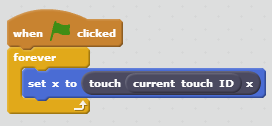
\includegraphics[width=0.4\textwidth]{images/OnePlayerPongAID.PNG}
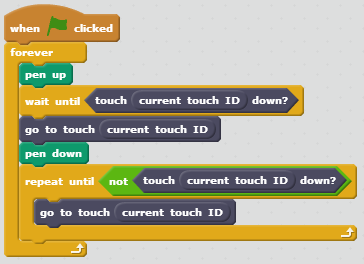
\includegraphics[width=0.59\textwidth]{images/OneFingerPaintingAID.PNG}
\caption[Sample Absolute Indexing Design Scripts for Low Floor Case Projects]{A sample Absolute Indexing Design script for the paddle controls in a one-player Pong game is on the left. On the right is a sample paintbrush script for one-finger painting.}
\label{LowFloorAID}
\end{figure}

By using the ``current touch ID" block to get the ID of the latest touch, both of the low floor case projects can be implemented in essentially the same way as was done using the previous two designs (Figure \ref{LowFloorAID}). Since we are assuming there is at most one touch on the screen at any time, the ``current touch ID" will always refer to the only touch on the tablet (if there is one).

Although these implementations look nearly as simple as those done with the Closest Finger Design, it might not be obvious to novice Scratchers that they can get access to the latest touch by inserting the ``current touch ID" block into the other touch blocks' (\emph{ID}) parameters. Blocks like ``touch (\emph{ID}) x" by themselves are neither tinkerable nor explorable, so it is difficult for Scratchers to learn how to use them without outside instruction. Unless the given (\emph{ID}) value happens to be an ID of one of the current touches, many of the Absolute Indexing Design blocks will appear unresponsive to touches.

One idea, to make the Absolute Indexing Design more explorable, would be for the block palette to feature  ``touch (\emph{ID}) x" and ``touch (\emph{ID}) y" blocks with the ``current touch ID" block already inserted in their (\emph{ID}) parameter. While this would definitely increase the explorability of the blocks, it could cause some confusion, because preassembled blocks have never before been featured in Scratch.


\subsection{Middle Height}

Once Scratchers get over the barrier of learning the intuition behind the  absolute indexing logic, they can, without too much difficulty, figure out how to implement both of the middle height case projects.

\begin{figure}
\centering
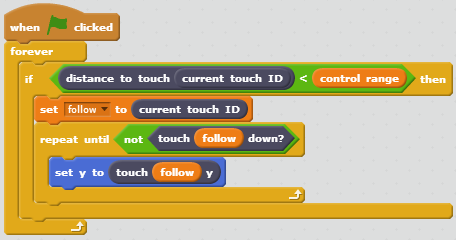
\includegraphics{images/BasicTwoPlayerPongAID.PNG}
\caption[Sample Absolute Indexing Design Script for Basic Two-Player Pong]
{Here is a sample script for controlling the paddle in a basic two-player Pong game using the Absolute Indexing Design.}
\label{BasicTwoPlayerPongAID}
\end{figure}

To begin, the controls for the basic two-player Pong game can be implemented by having both paddles constantly repeating a simple process (Figure \ref{BasicTwoPlayerPongAID}). First, each paddle's script can check to see if the touch with the ``current touch ID" is within their paddle's control range and store the ID in a variable if it is. Then, with the stored touch ID, the script can set the paddle to follow the touch with the stored ID until it is lifted.

Although this implementation of the basic two-player Pong game is complicated by the necessary use of a variable, experienced Scratchers generally have a basic understanding of how to use variables. As a result, barring the difficulty of understanding how the absolute indexing works, the complexity of this implementation is appropriate for a middle height project.

Like the basic two-player Pong game, the two-finger painting project can also be implemented using the Absolute Indexing Design by programming both of the paintbrushes to forever repeat a simple process while keeping a variable in which they store the ID of the touch they currently are following (Figure \ref{TwoFingerPaintingAID}). To begin each iteration of the repeated process, each paintbrush first checks to see if the touch with the ``current touch ID" is down and not being followed by the other paintbrush. If both criteria are met, then the paintbrush sets its variable to the current touch ID (thus claiming it) and follows the touch with its pen down until the touch is lifted.

\begin{figure}
\centering
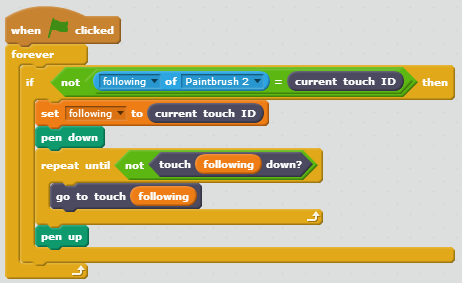
\includegraphics{images/TwoFingerPaintingAID.PNG}
\caption[Sample Absolute Indexing Design Script for Two-Finger Painting]
{Here is a sample script for controlling one of the paintbrushes in a two-finger painting project using the Absolute Indexing Design.}
\label{TwoFingerPaintingAID}
\end{figure}

Note that this implementation does rely on some of the specifics regarding Scratch's thread-switching protocol. However, the naive assumption that there will not be any race conditions in this case turns out to be true. As a result, this implementation is not too complicated for a middle height project. It is particularly noteworthy that two-finger painting can be implemented perfectly using the Absolute Indexing Design with an implementation that is no more complex as the imperfect implementations that could be created using the other two designs.

\subsection{High Ceiling}

When using the Absolute Indexing Design, the gap in complexity between the middle height and high ceiling case projects disappears. Once Scratchers have gained an intuition for how to use the Absolute Indexing Design to make multi-touch interactions with moderate complexity (which, granted, can be an arduous task), it becomes a natural and iterative process for them to discover how to make more complex ones.

\begin{figure}
\centering
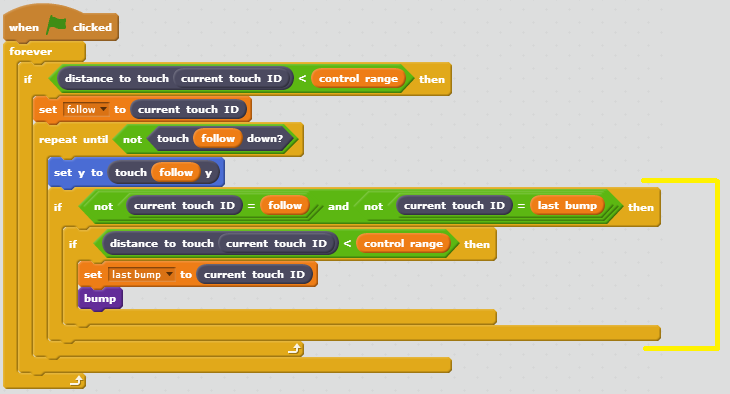
\includegraphics[width=0.8\textwidth]{images/AdvancedTwoPlayerPongAID.PNG}
\caption[Sample Absolute Indexing Design Script for Advanced Two-Player Pong]{Here is a sample script for controlling the paddle in an advanced two-player Pong game using the Absolute Indexing Design. The subroutine that is added to the basic two-player Pong game is highlighted. }
\label{AdvancedTwoPlayerPongAID}
\end{figure}

For example, the progression from the basic two-player Pong game to the advanced two-player Pong game is a particularly natural one when using the Absolute Indexing Design. To add the new bump interaction, each paddle's script can be augmented with an additional variable and a simple subroutine to be run when the paddle is following a particular touch (Figure \ref{AdvancedTwoPlayerPongAID}). The additional variable is used to store the ID of the touch that triggered the last bump, so that the same touch cannot trigger multiple bumps. Thus, the subroutine just checks on the current touch to see if it is different from both the touch the paddle is following and the touch that triggered the last bump. If both criteria are met, the subroutine makes a final check to see that the current touch is within the paddle's control range and initiates a bump if that is the case.

Similarly, the implementation for two-finger painting using the Absolute Indexing Design can easily be upgraded to ten-finger painting by simply adding more paintbrush sprites and more checks in each of their scripts to make sure that no paintbrush follows an already followed touch (Figure \ref{TediousMultiFingerPainting}). While this is an extremely simple augmentation, the script copying can become tedious. 

\begin{figure}
\centering
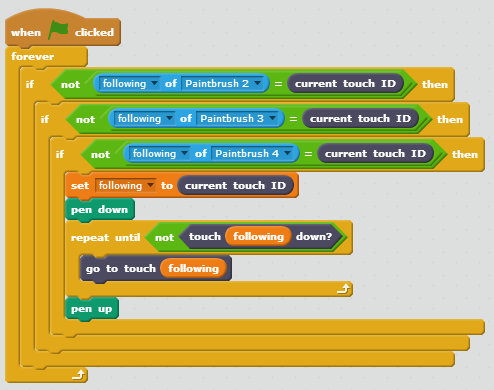
\includegraphics[width=0.6\textwidth]{images/TediousMultiFingerPainting.PNG}
\caption[Sample Absolute Indexing Design Script for Multi-Finger Painting]
{Here is a sample script for a paintbrush sprite in a four-finger painting project using the Absolute Indexing Design, but without using clones. To add more fingers, one need only add the additional paintbrush sprites and if statements.}
\label{TediousMultiFingerPainting}
\end{figure}

Hence, an experienced Scratcher may be tempted to use Scratch's cloning feature to make the implementation more elegant. Using the ``when touch created" block, a Scratcher can create a new paintbrush clone specifically to follow each new touch. The paintbrush clone would then follow its assigned touch until the touch is lifted, at which point the clone selflessly kills its own script to preserve computational resources. While the implementation using cloning is more elegant and uses fewer blocks, both implementations have the same functionality.

In comparison to the other two designs I have presented, the Absolute Indexing Design has a steep learning curve. It is very unlikely that someone could quickly figure out how the design's blocks work just by playing around with them. However, as multi-touch interactions become more complex, it becomes easier to implement them using the Absolute Indexing Design than with the other two designs.  

